\section{Синтез систем управления}\label{part_control_systems}
\subsection{Предварительные замечания}
Каждый из приводов манипулятора робота Kuka Youbot имеет собственную систему управления, структура которой иллюстрируется схемой с рисунка~\ref{img_structure_of_actuator_cs}.
Из нее видно, что каждый из приводов робота может управляться заданием значения для угла~$q_{di}$, или скорости~$\dot{q}_{di}$, или момента силы $\tau_{ed,i}$, который должен быть на нем обеспечен.
Это значение подается на вход соответствующего ПИД-регулятора, коэффициенты которого доступны настройке, и далее (уже в виде сигнала напряжения $u$)~--- на контролируемый двигатель.

\vspace{0.5cm}

\begin{figure}[h!]
	\centering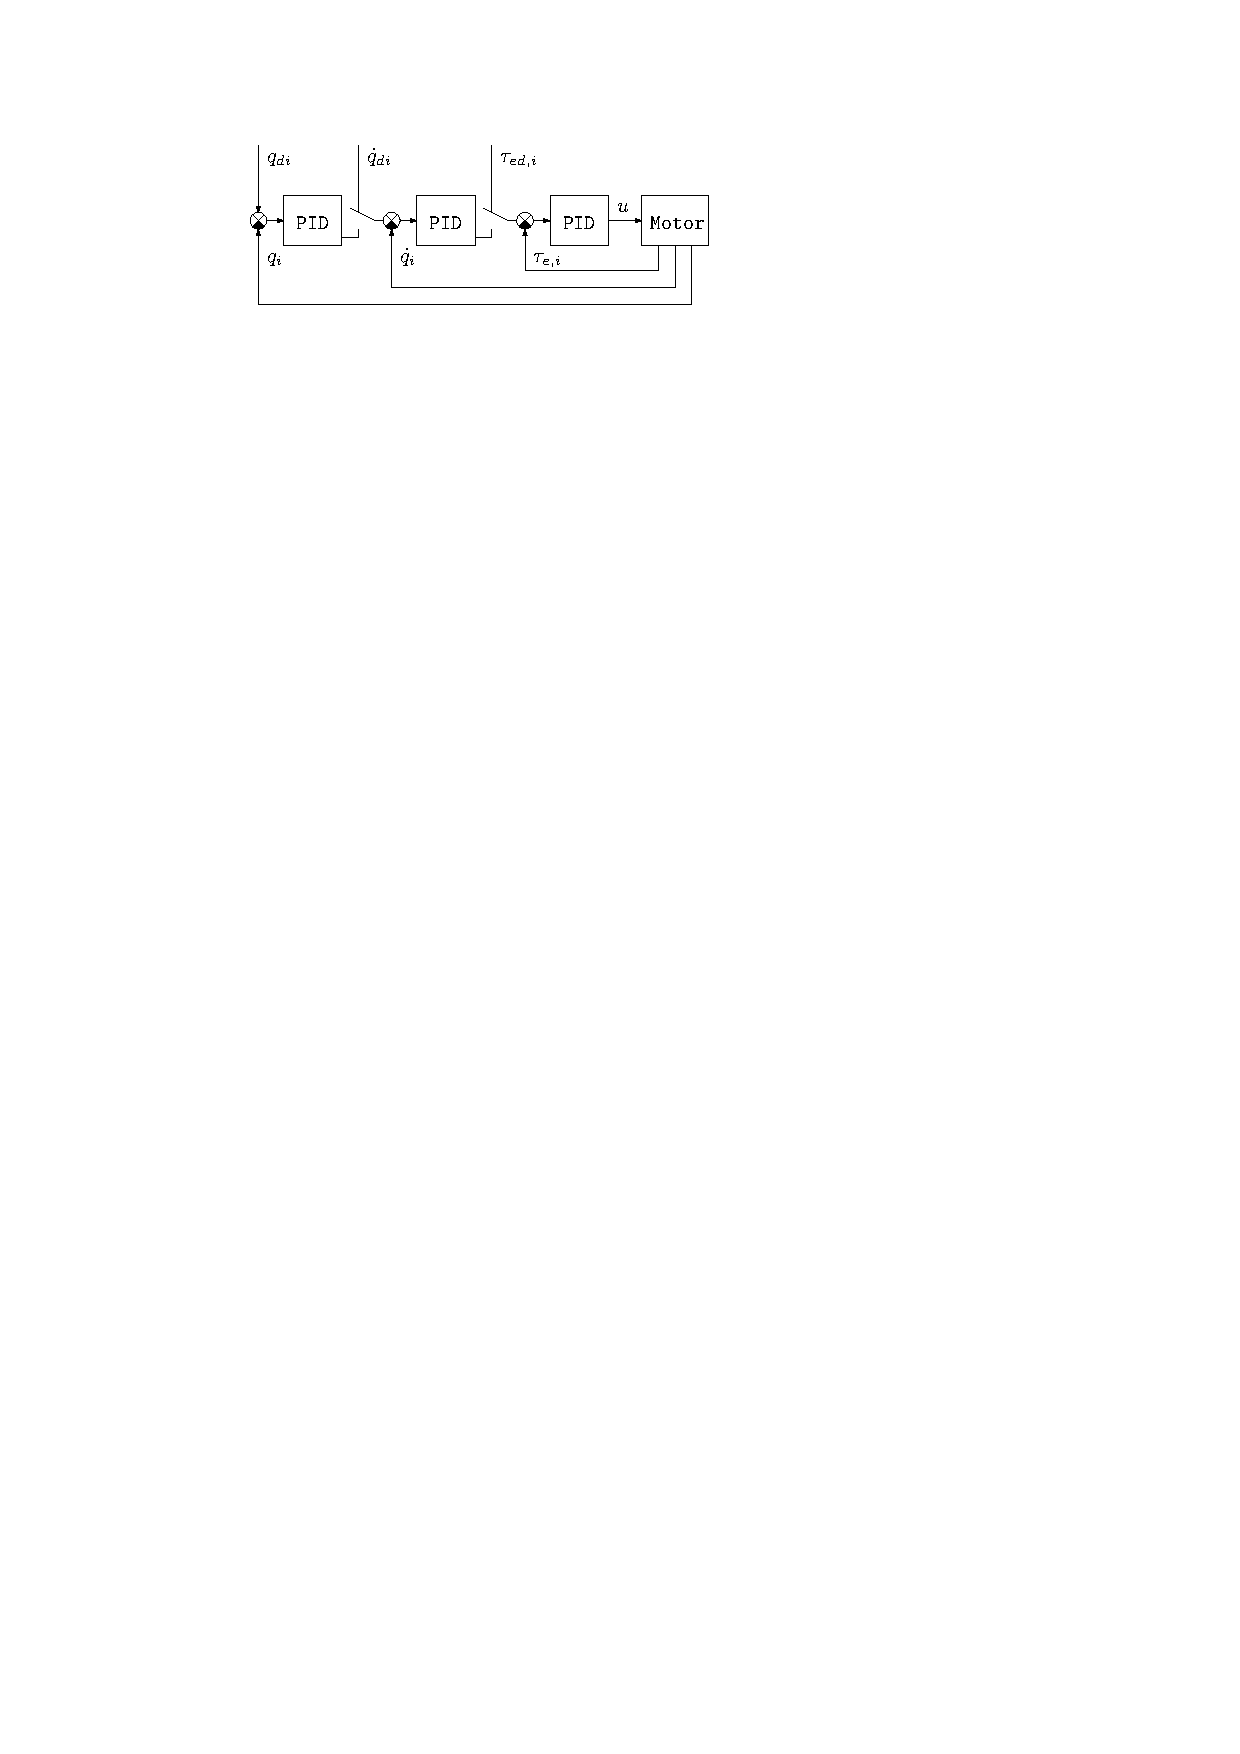
\includegraphics[width=0.8\textwidth]{structure_of_actuator_cs.pdf}
	\caption{Структура системы управления, контролирующей работу каждого из приводов робота.}
	\label{img_structure_of_actuator_cs}
\end{figure}

Далее в тексте документа будут рассмотрены системы управления, в которых в качестве управляющего сигнала рассматривается вектор $\tau_e(t)$.
При этом будет предполагаться, что задаваемые значения для моментов сил достигаются на двигателях мгновенно.
Такое предположение будем считать возможным по той причине, что процессы в контуре момента в рассмотренной выше системе управления характеризуются малыми временами переходных процессов.
В~качестве иллюстрации к сказанному можно привести рисунок~\ref{img_pid_transition_function}.
На нем показан график переходной функции системы управления моментом силы, развиваемым приводом ???-го звена.

\begin{figure}[h!]
	\centering\includegraphics[width=0.5\textwidth, draft]{pid_transition_function.pdf}
	\caption{График переходной функции системы управления приводом ???-го звена.}
	\label{img_pid_transition_function}
\end{figure}

Из величин, описывающих состояние робота в данный момент времени, в используемом ПО доступны вектора $q(t)$, $\dot{q}(t)$ и $\tau_e(t)$.

\newpage
